\section{Classes} \label{sc:classes}
The interviews with the client, made it possible to define the objects in the problem domain, and the relationships between them. This is illustrated in a class diagram (figure \ref{fig:ClassDiagram}).

% Figur af klassediagrammet
\begin{figure}[H]
    \centering
    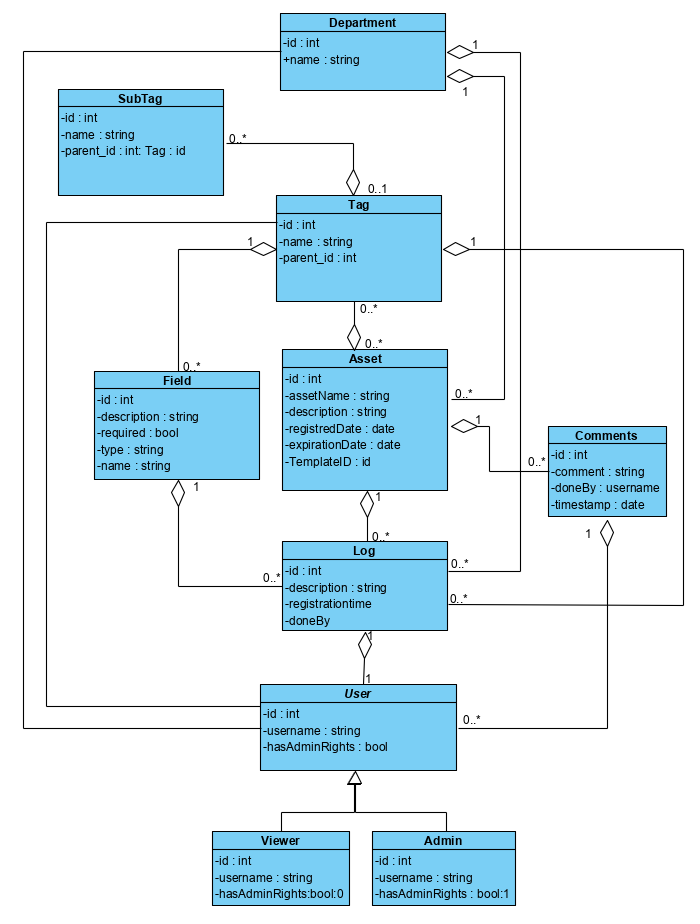
\includegraphics[width=1.0\textwidth]{figures/ClassDiagramV3.png}
    \caption{Class diagram of the objects in the problem domain.}
    \label{fig:ClassDiagram}
\end{figure}

% Beskriv den overordnede ide med systemet ud fra klassediagrammet?

% In figure \ref{fig:ClassDiagram} the connections between a number of classes is shown. These classes are describes as such: \par

The system is developed to support assets with different \textit{tags} attached. An \textit{asset} is, in the context of this project, understood as any physical item, or license belonging to a \textit{department}. A \textit{department} represents a department at the Zoo, and is implemented to function as a group of \textit{assets}, so a user can search for \textit{assets} in a specific \textit{department}.
\par
\textit{tag} is an identifier, which makes it possible to group assets. An \textit{Asset} contains zero or more tags and a \textit{tag} can be attached to zero or more \textit{assets}. This depicts a many-to-many relation between the two classes, which enables multiple assets with the same tag, and multiple tags attached to the same asset. A \textit{tag} can add a number of \textit{fields} to the asset it is attached to. These \textit{fields} can then be filled out by the user, providing additional information about the \textit{asset} dynamically. Some \textit{fields} may be required to be filled out.
Tags can be grouped and managed using supertags/subtags. A tag becomes a sub tag, when it has a relation to another tag.
\todo{Subtags/supertags relationen - måske skrevet} 

\subsection{State change diagrams}

\begin{figure}[H]
    \centering
    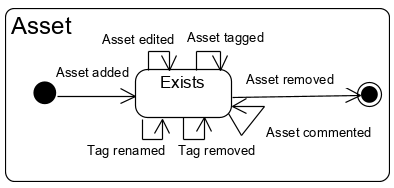
\includegraphics{figures/Asset_statechart.png}
    \caption{Statechart diagram for Asset}
    \label{fig:asset_statechart}
\end{figure}

Throughout the lifetime of an asset it only has a few connected events. After it has been created it can be modified in different ways. 
\begin{itemize}
    \item Asset can be edited, this can include, name changes.
    \item Asset tagged, this links a tag to the asset.
    \item Tag renamed, this gives one of the connected tags a new name.
    \item Tag removed(Asset untagged) this disconnects the link between the asset and a tag.
    \item Asset commented, this event is triggered when a user leaves a comment on the asset.
\end{itemize}
The assets lifetime ends when the asset is removed from the database, and is therefor no longer getting tracked. The statechart for an asset, can be seen on \ref{fig:asset_statechart}.

\begin{figure}[H]
    \centering
    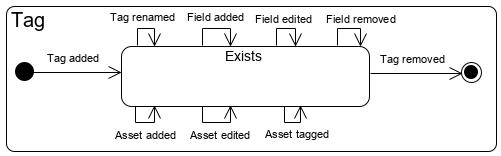
\includegraphics{figures/Tag_statechart.png}
    \caption{Statechart diagram for Tag}
    \label{fig:tag_statechart}
\end{figure}

The lifetime of a tag begins when a tag is added to the system. An existing tag can be affected by several events. For example when changes are made to the tag itself, or associated fields and assets. The lifetime of a tag ends when it is removed from the system. The statechart for the behavior of the tag class, is demonstrated in figure \ref{fig:tag_statechart}.

\begin{figure}[H]
    \centering
    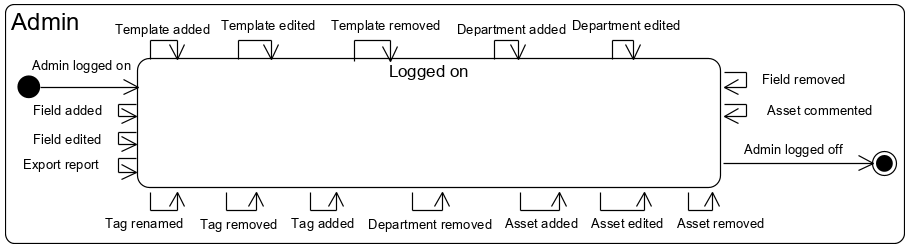
\includegraphics[width=14cm]{figures/Admin_statechart.png}
    \caption{Statechart diagram for Admin}
    \label{fig:admin_statechart}
\end{figure}

The admin class has a larger number of possible events, as this is a user with privileges to make changes in the system. An admin object is created when a user with administrator privileges logs in to the system. Then it is possible to add or remove objects, or edit those that are already present in the system. For example it is possible to add, remove, or edit tags on a particular asset, or comment on an asset. It is also possible for an admin to get a log of all the changes that has been made in the system. An administrator object is terminated when the user with administrator privileges logs off the system. This behavior is illustrated in figure \ref{fig:admin_statechart}.

\begin{figure}[H]
    \centering
    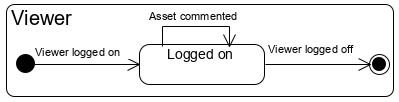
\includegraphics{figures/Viewer_statechart.png}
    \caption{Statechart diagram for Viewer}
    \label{fig:viewer_statechart}
\end{figure}

\begin{figure}[H]
    \centering
    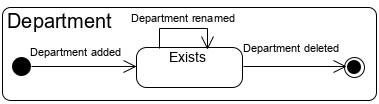
\includegraphics{figures/Department_statechart.png}
    \caption{Statechart diagram for Department}
    \label{fig:department_statechart}
\end{figure}

\begin{figure}[H]
    \centering
    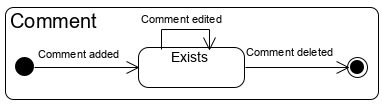
\includegraphics{figures/Comment_statechart.png}
    \caption{Statechart diagram for Comment}
    \label{fig:comment_statechart}
\end{figure}

\begin{figure}[H]
    \centering
    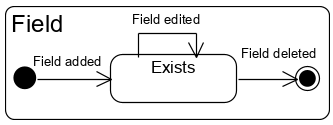
\includegraphics{figures/Field_statechart.png}
    \caption{Statechart diagram for Field}
    \label{fig:field_statechart}
\end{figure}

The classes Viewer, Department, Comment and Field all have similar behavior. As figures \ref{fig:viewer_statechart}, \ref{fig:department_statechart}, \ref{fig:comment_statechart} and \ref{fig:field_statechart} show, the objects are created either when they are added by an admin, or in the case of a Viewer, when a user without administrator privileges logs in. Then the only possible event is the editing of the object. The objects are terminated when they are removed from the system, or when they log off in the case of a Viewer.